In this report, we have analyzed the supply and demand of meeting rooms and toilet facilities for different campuses across the University of Melbourne based on our Non-randomized Anytime Orienteering Algorithm. To meet different requirements and situations when either a meeting room or a toilet facility is needed, we introduced different factors in our algorithm. Therefore, it will find the best results depending on the specific needs. 

We have done researches on the most demanding buildings and have obtained desirable results. When different factors such as COVID-19 lockdown, easy availability, and high capacity are incorporated, we can get different advice from our algorithm to guide us to find the best buildings and floors. \texttt{Doug McDonell Building} is a good example here. With no preference provided, \texttt{University Health Services Building}, \texttt{Kenneth Myer Building}, and \texttt{Old Physics Building} are the most rewarding buildings to book a meeting room.

Hence, when different requirements were passed to our algorithm, we can find the most suitable buildings for university staff who wants to book a meeting room or a student who wants to use toilet facility in the nearby buildings or even within the building that can meet those requirements. \texttt{University Spatial Analytics and Space Management} department can use this information to plan and allocate meeting room and toilet resources efficiently to better utilize them without occurring extra expenses.

As an achievement, we submitted our novel algorithm as a research paper[\ref{rpaper}] in AAAI 21 student abstract program's constraint satisfaction problem track as shown below.

\begin{figure}[H]
\centering
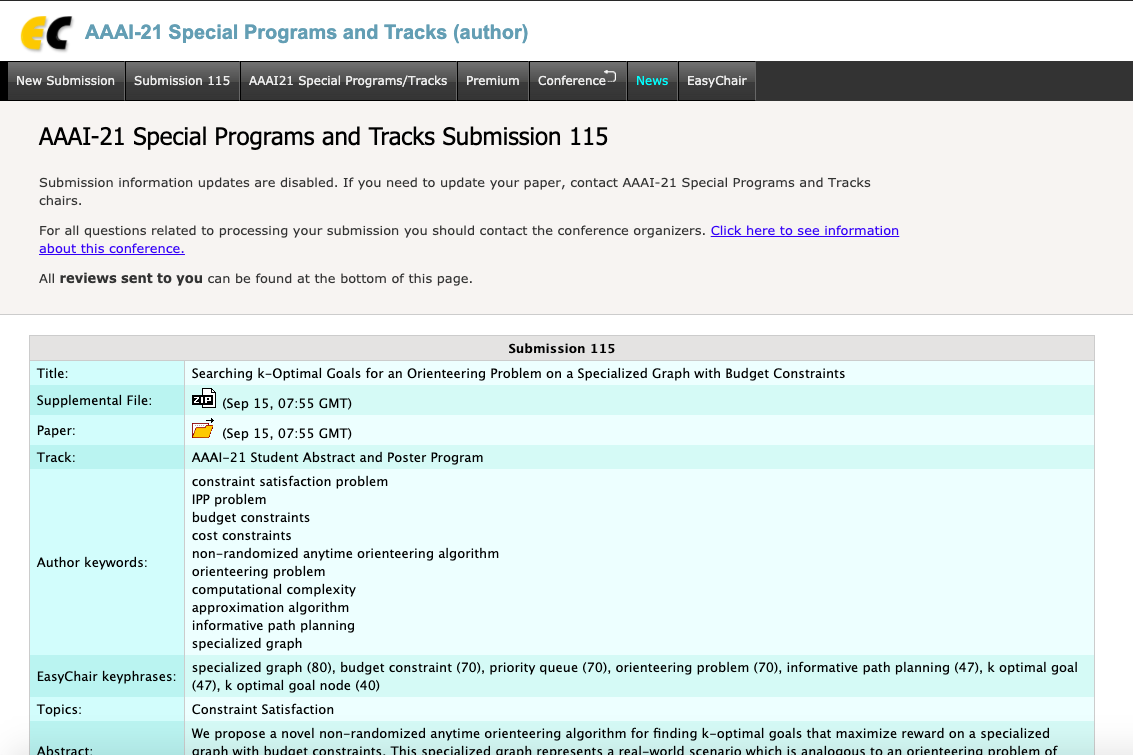
\includegraphics[width=14cm]{resources/images/achieve1.png}
\caption{AAAI 21 Student Abstract Program Submission}
\label{fig:achieve1}
\end{figure}

Unfortunately, our submission was not selected but we received valuable feedback that can be used for continuing research on this problem. In the end, we successfully published our research in the Cornell arXiv as shown with the link below.

\begin{figure}[H]
\centering
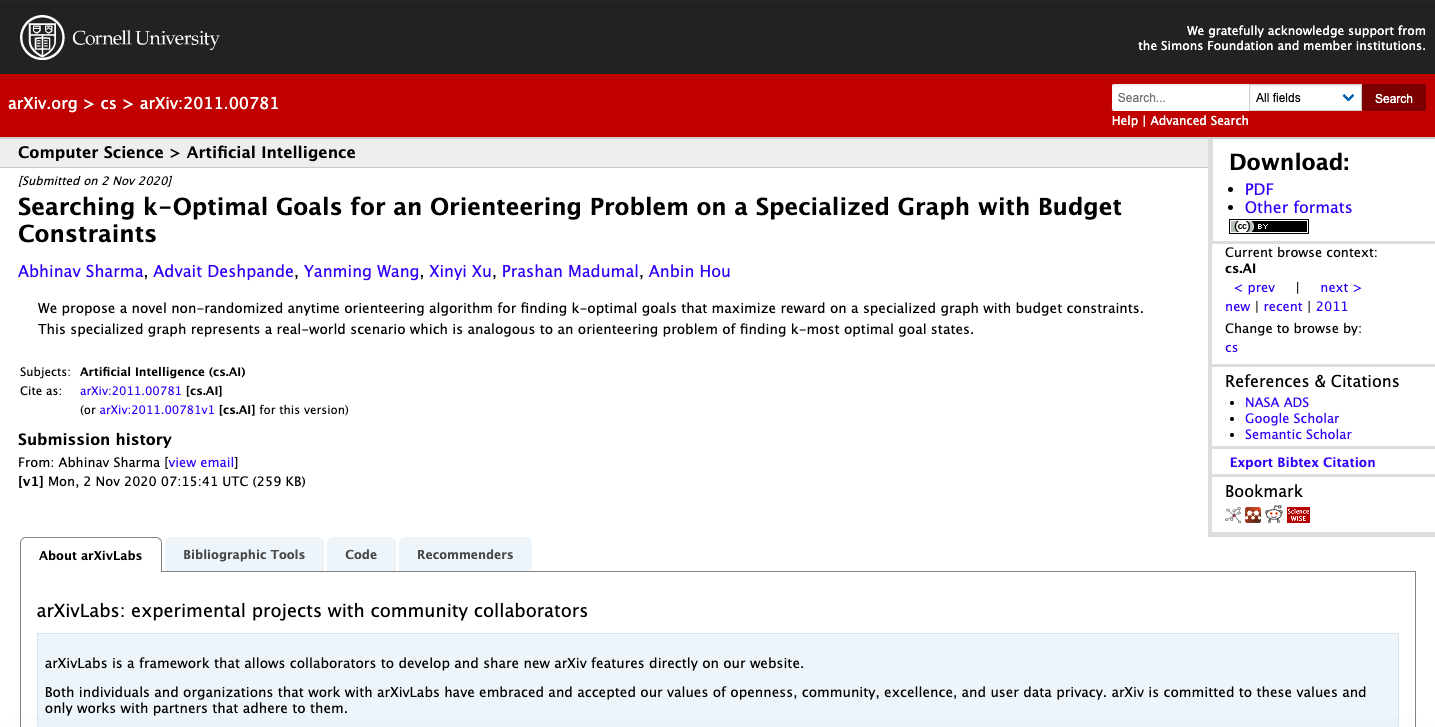
\includegraphics[width=15cm]{resources/images/achieve2.png}
\caption{Research published in arXiv: \url{https://arxiv.org/abs/2011.00781}}
\label{fig:achieve2}
\end{figure}

In conclusion, our non-randomized anytime orienteering algorithm is not limited to solve the spatial optimization problem only as it is a generalized algorithm that can be expanded to other areas as well. This will require further studies.